\chapter{System Design}
\begin{sidewaysfigure}
  \begin{center}
    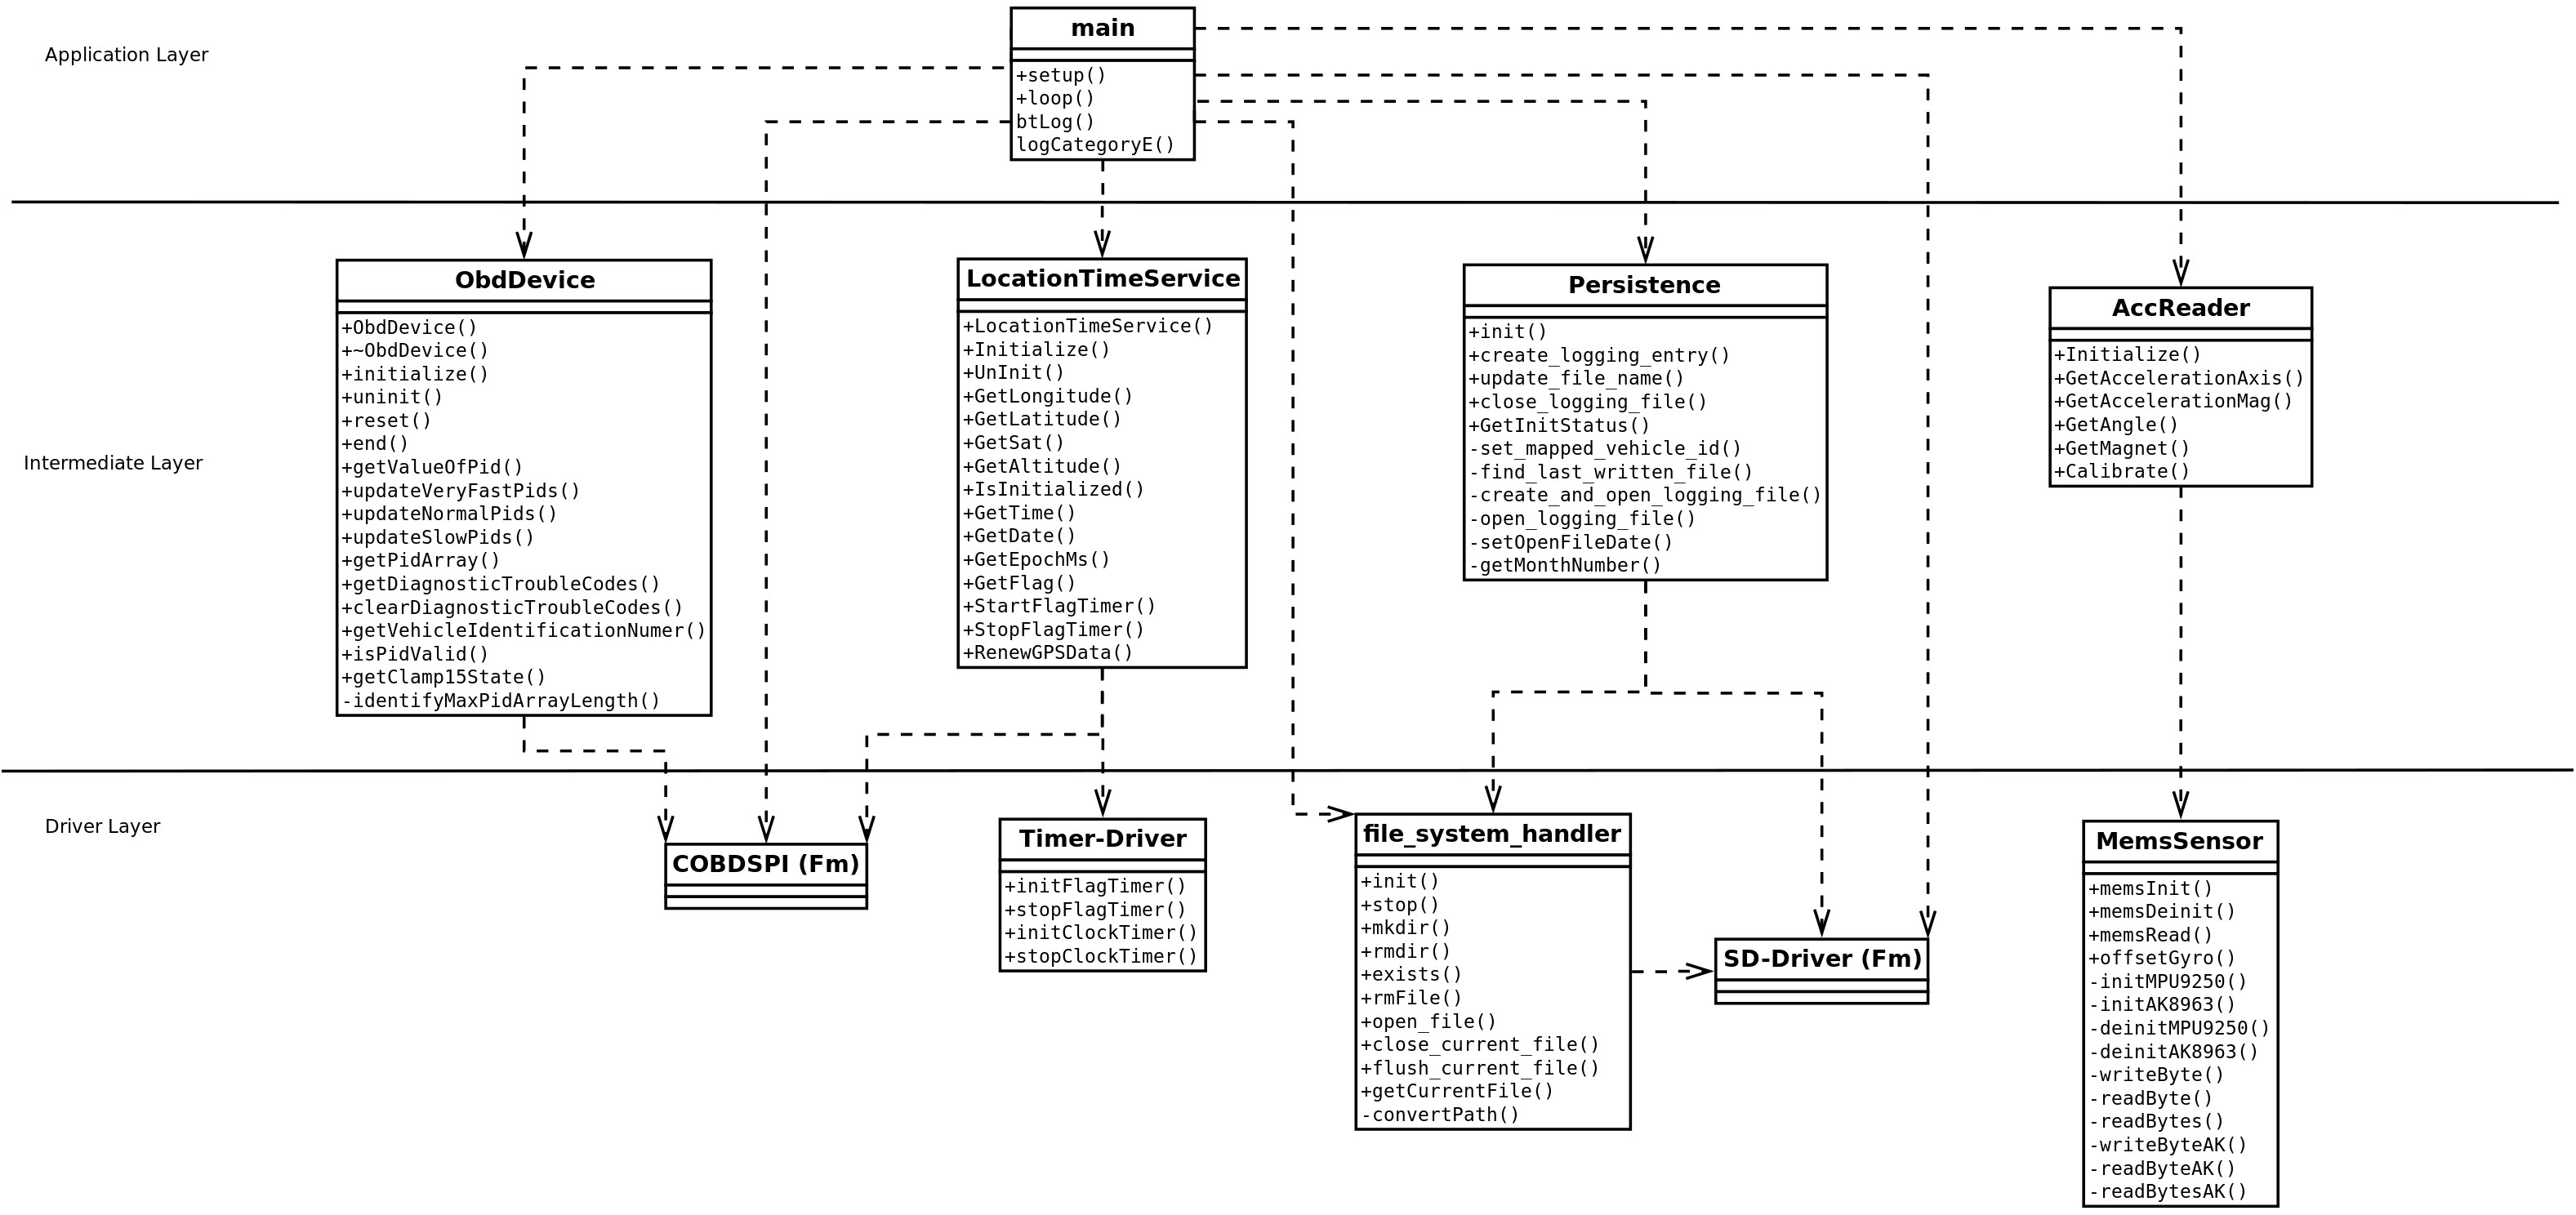
\includegraphics[width=\textwidth,height=15cm,keepaspectratio]{./img/Dongle_Arch_final}
    \caption{Architektur der Dongle-Software}
    \label{fig:dongleArch}
  \end{center}
\end{sidewaysfigure}
\section{Dongle}
Wie auf der Produkthomepage beschrieben, so nutzt der Dongle als Haupt-Controller einen ATmega328p, wie er auch auf einem Arduino UNO verwendet wird. Bei der Architektur der Dongle-Software wird deshalb für den Programmablauf ein für Arduino-Projekte klassischer Aufbau mit einer ``setup''- und einer ``loop''-Funktion innerhalb einer main-Datei verwendet.
\paragraph{}
Um bei der Entwicklung der Software für den Dongle möglichst wenig Inhaltsüber-schneidungen der Teammitglieder zu erreichen und um die Verständlichkeit und Wartbarkeit des Codes zu verbessern wurde entschieden die Schichtenarchitektur wie in Bild \ref{fig:dongleArch} umzusetzen.

Hierbei wird für die meisten Funktionsmerkmale mindestens eine Klasse auf der Intermediate-Layer sowie der Driver-Layer implementiert. Dies hat zur Folge, dass bei einer Funktionsänderung wie beispielsweise der Verwendung eines anderen GPS-Empfängers nur die entsprechende Treiber-Klasse geändert werden muss. Die Hauptklasse mit der eigentlichen Programmlogik bleibt dabei unangetastet.\\
Die im Bild \ref{fig:dongleArch} mit ``(Fm)'' ergänzten Klassen werden aus den Bibliotheken des Herstellers übernommen.
\subsection{Programmlogik}
Die eigentliche Programmlogik kann wie bereits erwähnt in die Teile ``Setup'' und ``Loop'' getrennt werden.
\begin{figure}
  \begin{center}
    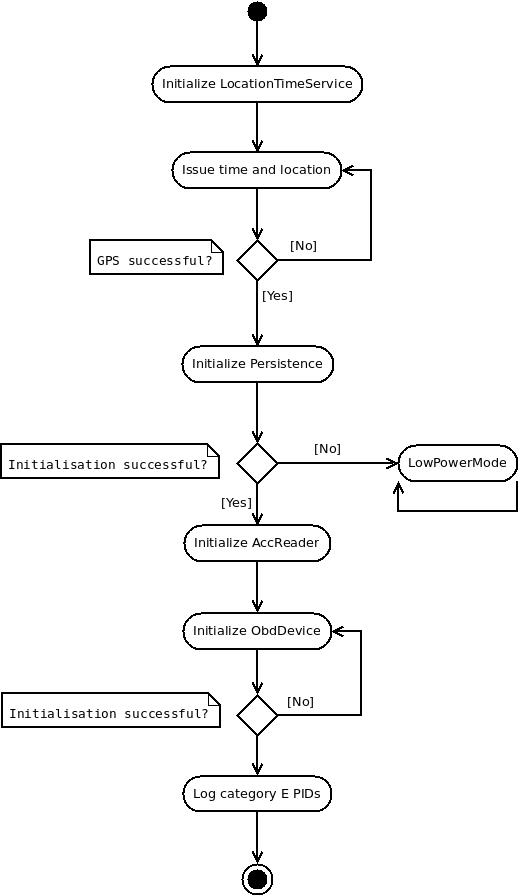
\includegraphics[width=\textwidth,height=20cm,keepaspectratio]{./img/Startup}
    \caption{Programmablauf der Initialisierung}
    \label{fig:setup}
  \end{center}
\end{figure}
\paragraph{}
Die Abbildung \ref{fig:setup} beschreibt den Ablauf des Programms beim Einstecken des Adapters in die Schnittstelle des Autos. Hervorzuheben ist, dass die Reihenfolge der Initialisierungen von großer Bedeutung ist. Während der Integration zeigte sich, dass die Persistenz-Klasse zur Initialisierung wesentlich mehr RAM benötigt als während des normalen Programmablaufs. Deshalb muss diese so früh wie möglich initialisiert werden. Nur die Klasse für GPS und Zeit muss zuvor bereit sein, da die Persistenzklasse diese während der Initialisierung aufruft.
\begin{figure}
  \begin{center}
    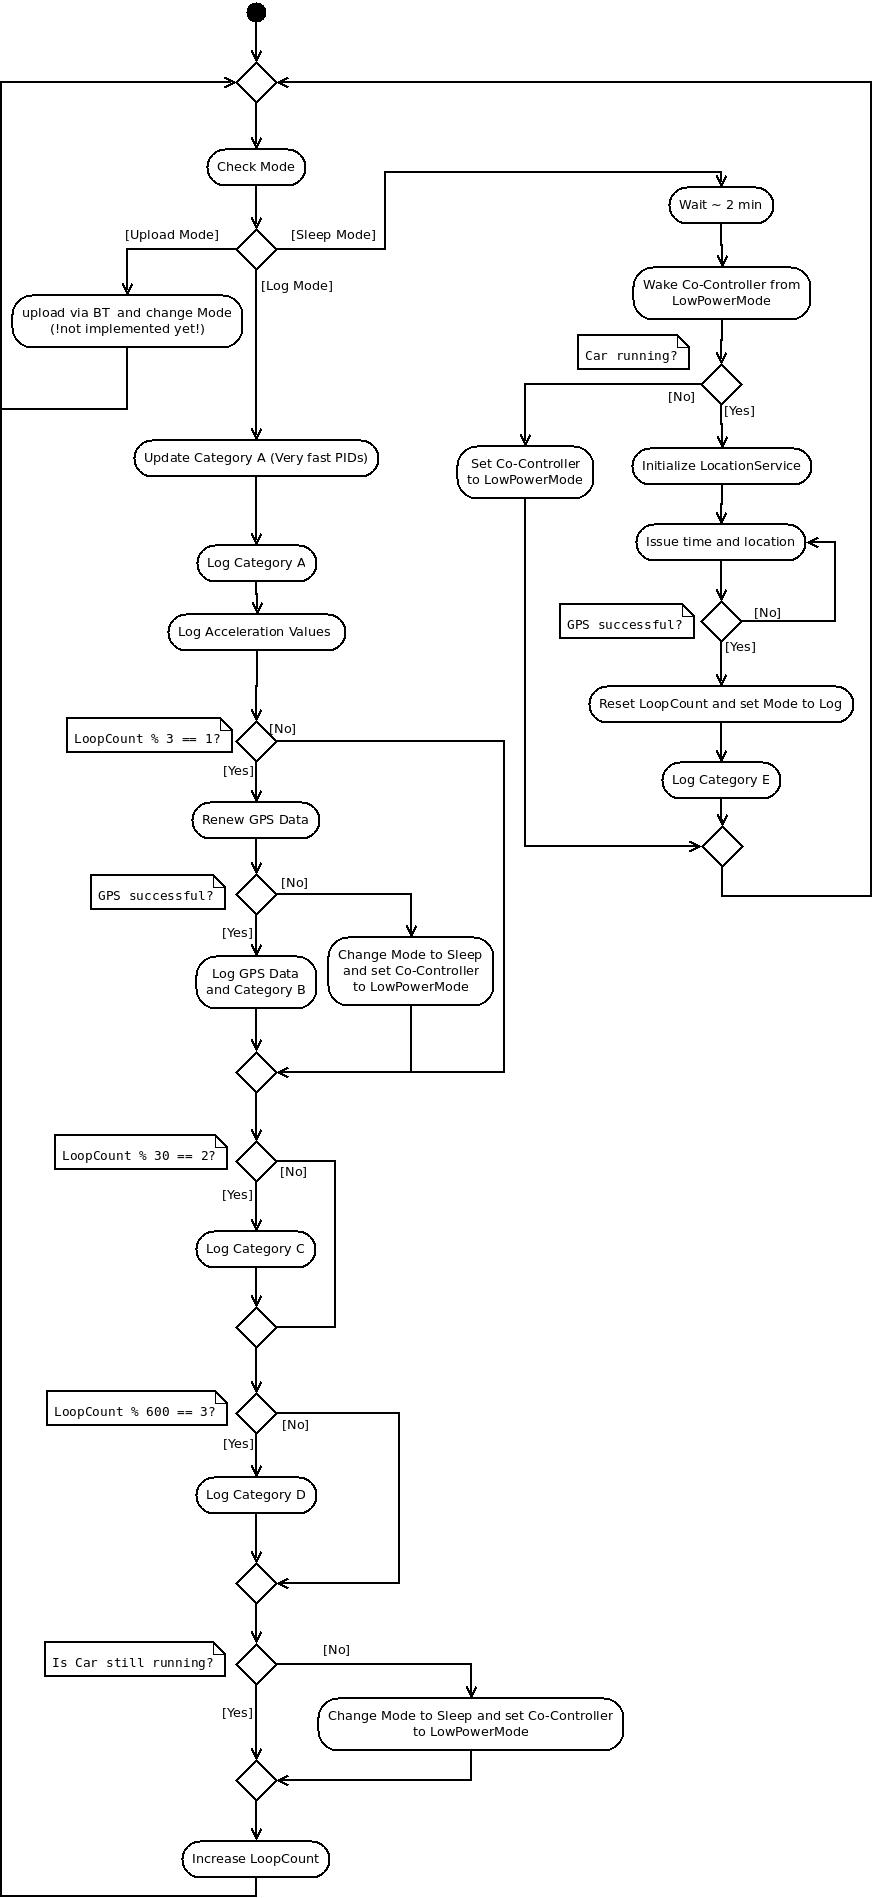
\includegraphics[width=\textwidth,height=20cm,keepaspectratio]{./img/ProgLoop}
    \caption{Programmablauf der Endlosschleife}
    \label{fig:loop}
  \end{center}
\end{figure}
In Abbildung \ref{fig:loop} ist der Ablauf des Programms ersichtlich, welches die eigentliche Funktionalität enthält. Dies wurde in drei Modi umgesetzt. Während des Logging-Modus werden die Fahrzeug-Daten gesammelt, auf eine SD-Karte geschrieben und per Bluetooth an ein Smartphone gesandt. Der Upload-Modus dient dazu, die gesammelten Daten auf der SD-Karte an die Smartphone-App weiterzugeben. Dies soll ein Entnehmen der Karte zum Auslesen der Daten optional machen. Der Schlafmodus dient letztendlich dazu, bei abgeschalteter Zündung das Bordnetz des Fahrzeugs möglichst wenig zu belasten.
\subsection{GPS-Empfänger}
Da ein zentrales Ziel der Applikation die Anfertigung eines Fahrtenbuches mit Streckenaufzeichnung ist, muss auch die Position des Fahrzeuges möglichst genau bestimmt werden. Der in diesem Projekt verwendete Freematics ONE bietet hier die Möglichkeit, einen externen GPS-Empfänger per UART anzubinden.
\paragraph{}
Um die Anschaffungskosten zu reduzieren, wurde zunächst untersucht, ob neben dem von Freematics verkauften GPS-Empfänger auch andere GPS-Receiver-Chips mit dem OBD-Dongle kompatibel sind.
Ein Problem bei dieser Untersuchung ist die Architektur des Freematics ONE, da die Kommunikation mit dem GPS-Empfänger nicht auf dem ATmega328p Haupt-Controller sondern auf einem STM32 Coprozessor ausgeführt wird. Leider ist der Code auf dem Coprozessor nicht öffentlich einsehbar und auch nicht ohne großen Aufwand auslesbar.
Ein weiteres Problem bestand darin, dass auch ein Öffnen des Gehäuses des von Freematics selbst vertriebenen GPS-Empfängers nicht zur Identifikation des Chips beitragen konnte. Es wurde allerdings klar, dass dieser nicht der Angabe auf der Produkthomepage des Freematics ONE entsprach. Der Empfänger-Chip ist nur mit einem QR-Code versehen und eine Recherche zum Hersteller verwies nur auf den chinesischen Produzenten des ganzen Empfänger-Moduls.(www.szgrltd.com)
\paragraph{}
Daher wurde eine andere Vorgehensweise zur Untersuchung der Kommunikation angewandt. Dazu wurde, wie in Abbildung \ref{fig:gpsAnalyse} abgebildet, ein zusätzlicher Arduino UNO als Zwischenstation in die UART-Kommunikation zwischen Dongle und Empfänger eingefügt. Zwei durch Software simulierte, serielle Schnittstellen auf dem Arduino UNO werden nun genutzt, um die vom Dongle und vom GPS-Empfänger gesendeten Daten aufzufangen, auf der über USB angeschlossenen seriellen Konsole eines Rechners auszugeben und an den jeweils anderen Kommunikationspartner weiterzuleiten.
\begin{figure}
  \begin{center}
    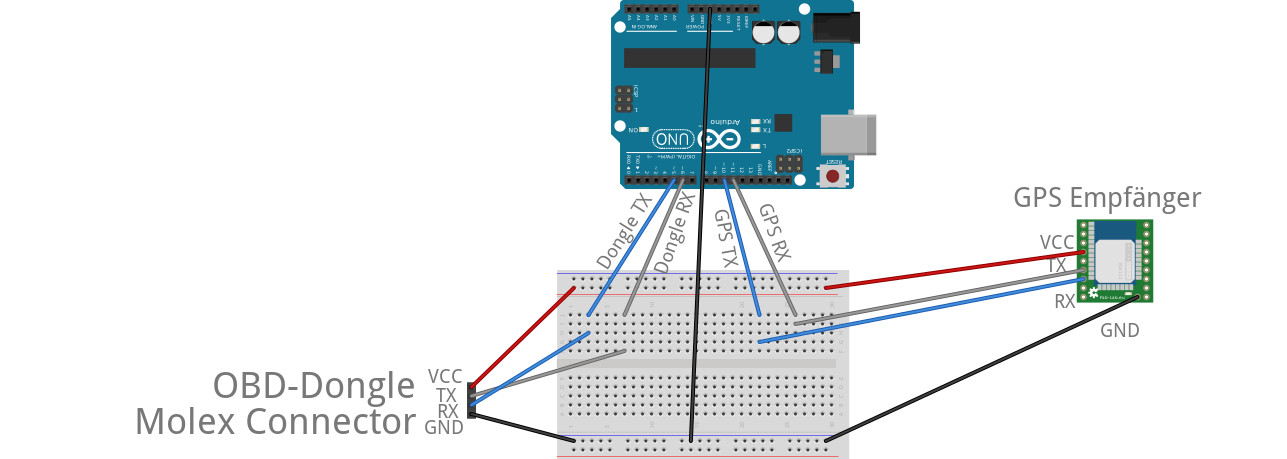
\includegraphics[width=\textwidth]{./img/gpsVersuch}
    \caption{Versuchsaufbau zur Analyse der UART-Kommunikation zwischen Dongle und GPS-Empfänger}
    \label{fig:gpsAnalyse}
  \end{center}
\end{figure}
\paragraph{}
Nach Auswertung der Kommunikation, stand fest, dass der von Freematics gelieferte Gps-Empfänger kompatibel zu einem u-blox UBX-G7020 ist. Dieser versendet standardmäßig Nachrichten gemäß dem NMEA Standard. Darüber hinaus wurde ersichtlich, dass der OBD-Dongle keine Nachrichten zum GPS-Chip sendet.
\paragraph{}
Da nun allerdings der konkrete Empfänger feststand, konnte dazu die entsprechende Protocol Specification heruntergeladen und mit weiteren GPS-Empfängern verglichen werden.
Letztendlich wurde ein Pixhawk GPS Empfänger für einen Modellbau-Quadrokopter auf Basis eines u-blox Neo6M mit zusätzlichem Magnetfeld-Sensor ausgewählt. Dieser Mikrochip verfügt zwar nicht über die exakt gleiche Protocol Specification, die ab Werk konfigurierte Kommunikation jedoch ist nahezu identisch und kompatibel mit der des von Freematics gelieferten Produktes.
\paragraph{}
Um den neuen Empfänger am Dongle zu betreiben, wurde an dessen Signal-Eingängen ein 2x2-Molex Stecker passend angelötet. Die I2C-Pins des Magnetfeld-Sensors wurden dabei nicht belegt.
\paragraph{}
Ein erster Test mit der mitgelieferten Software zeigte die grundsätzliche Funktion des neuen GPS-Moduls. Allerdings ist die Genauigkeit des Pixhawk-Empfängers etwas schlechter als die des UBX-G7020.
\subsection{Zeit}
Wie bereits erwähnt, muss auch auf dem Dongle eine Repräsentation der genormten Zeit vorhanden sein. Zunächst soll jeder erfasste Datenwert mit einem Zeitstempel versehen werden um mit einer totalen Ordnung die Analyse dieser Werte erst zu ermöglichen. Zum anderen sollen die Datenwerte mit einem Intervall von 200 Millisekunden erfasst werden.
\paragraph{}
Die Anforderung nach einem genauen Zeitintervall von 200 Millisekunden zwischen dem Abrufen der OBD-Werte der Klasse A kann durch den Einsatz eines Hardware-Timers und Interrupts gelöst werden.
Auf dem ATmega328p Hauptcontroller stehen dem Entwickler 3 Hardware-Timer zur Verfügung. Allerdings muss hierbei beachtet werden, dass die Arduino-Bibliothek den Timer 0 für die Funktionen delay() und millis() verwendet und diese daher unangetastet bleiben sollten.\cite{arduinoTimer}
Da die Intervalle zum Abrufen der PID-Klassen B, C und D ein Vielfaches der 200 Millisekunden der Klasse A sind, müssen für diese keine weiteren Timer verwendet werden. Statt dessen kann ein einfacher Vergleich in Kombination mit dem Modulo-Operator genutzt werden (vgl. Abbildung \ref{fig:loop}).
\subsection{Beschleunigungssensor}
Zunächst wurde ermittelt, welcher Sensor im Dongle verbaut wurde. Anhand der Informationen auf der Produkthomepage sowie des Source-Codes des Treibers wurde ersichtlich, dass ein MPU-9250 MEMS Bewegungssensor mit jeweils 3 Achsen für Beschleunigungs-, Drehraten- und Magnetfeldmessung verbaut ist. Hierbei ist besonders, dass der Sensor für das Magnetfeld als I²C-Submodul am Sensor ausgeführt ist.
